% Options for packages loaded elsewhere
\PassOptionsToPackage{unicode}{hyperref}
\PassOptionsToPackage{hyphens}{url}
\PassOptionsToPackage{dvipsnames,svgnames*,x11names*}{xcolor}
%
\documentclass[
  12pt,
]{article}
\usepackage{lmodern}
\usepackage{setspace}
\usepackage{amssymb,amsmath}
\usepackage{ifxetex,ifluatex}
\ifnum 0\ifxetex 1\fi\ifluatex 1\fi=0 % if pdftex
  \usepackage[T1]{fontenc}
  \usepackage[utf8]{inputenc}
  \usepackage{textcomp} % provide euro and other symbols
\else % if luatex or xetex
  \usepackage{unicode-math}
  \defaultfontfeatures{Scale=MatchLowercase}
  \defaultfontfeatures[\rmfamily]{Ligatures=TeX,Scale=1}
  \setmainfont[]{Times New Roman}
  \setsansfont[]{Times New Roman}
\fi
% Use upquote if available, for straight quotes in verbatim environments
\IfFileExists{upquote.sty}{\usepackage{upquote}}{}
\IfFileExists{microtype.sty}{% use microtype if available
  \usepackage[]{microtype}
  \UseMicrotypeSet[protrusion]{basicmath} % disable protrusion for tt fonts
}{}
\makeatletter
\@ifundefined{KOMAClassName}{% if non-KOMA class
  \IfFileExists{parskip.sty}{%
    \usepackage{parskip}
  }{% else
    \setlength{\parindent}{0pt}
    \setlength{\parskip}{6pt plus 2pt minus 1pt}}
}{% if KOMA class
  \KOMAoptions{parskip=half}}
\makeatother
\usepackage{xcolor}
\IfFileExists{xurl.sty}{\usepackage{xurl}}{} % add URL line breaks if available
\IfFileExists{bookmark.sty}{\usepackage{bookmark}}{\usepackage{hyperref}}
\hypersetup{
  colorlinks=true,
  linkcolor=Maroon,
  filecolor=Maroon,
  citecolor=Blue,
  urlcolor=Blue,
  pdfcreator={LaTeX via pandoc}}
\urlstyle{same} % disable monospaced font for URLs
\usepackage[margin=1in]{geometry}
\usepackage{color}
\usepackage{fancyvrb}
\newcommand{\VerbBar}{|}
\newcommand{\VERB}{\Verb[commandchars=\\\{\}]}
\DefineVerbatimEnvironment{Highlighting}{Verbatim}{commandchars=\\\{\}}
% Add ',fontsize=\small' for more characters per line
\usepackage{framed}
\definecolor{shadecolor}{RGB}{248,248,248}
\newenvironment{Shaded}{\begin{snugshade}}{\end{snugshade}}
\newcommand{\AlertTok}[1]{\textcolor[rgb]{0.94,0.16,0.16}{#1}}
\newcommand{\AnnotationTok}[1]{\textcolor[rgb]{0.56,0.35,0.01}{\textbf{\textit{#1}}}}
\newcommand{\AttributeTok}[1]{\textcolor[rgb]{0.77,0.63,0.00}{#1}}
\newcommand{\BaseNTok}[1]{\textcolor[rgb]{0.00,0.00,0.81}{#1}}
\newcommand{\BuiltInTok}[1]{#1}
\newcommand{\CharTok}[1]{\textcolor[rgb]{0.31,0.60,0.02}{#1}}
\newcommand{\CommentTok}[1]{\textcolor[rgb]{0.56,0.35,0.01}{\textit{#1}}}
\newcommand{\CommentVarTok}[1]{\textcolor[rgb]{0.56,0.35,0.01}{\textbf{\textit{#1}}}}
\newcommand{\ConstantTok}[1]{\textcolor[rgb]{0.00,0.00,0.00}{#1}}
\newcommand{\ControlFlowTok}[1]{\textcolor[rgb]{0.13,0.29,0.53}{\textbf{#1}}}
\newcommand{\DataTypeTok}[1]{\textcolor[rgb]{0.13,0.29,0.53}{#1}}
\newcommand{\DecValTok}[1]{\textcolor[rgb]{0.00,0.00,0.81}{#1}}
\newcommand{\DocumentationTok}[1]{\textcolor[rgb]{0.56,0.35,0.01}{\textbf{\textit{#1}}}}
\newcommand{\ErrorTok}[1]{\textcolor[rgb]{0.64,0.00,0.00}{\textbf{#1}}}
\newcommand{\ExtensionTok}[1]{#1}
\newcommand{\FloatTok}[1]{\textcolor[rgb]{0.00,0.00,0.81}{#1}}
\newcommand{\FunctionTok}[1]{\textcolor[rgb]{0.00,0.00,0.00}{#1}}
\newcommand{\ImportTok}[1]{#1}
\newcommand{\InformationTok}[1]{\textcolor[rgb]{0.56,0.35,0.01}{\textbf{\textit{#1}}}}
\newcommand{\KeywordTok}[1]{\textcolor[rgb]{0.13,0.29,0.53}{\textbf{#1}}}
\newcommand{\NormalTok}[1]{#1}
\newcommand{\OperatorTok}[1]{\textcolor[rgb]{0.81,0.36,0.00}{\textbf{#1}}}
\newcommand{\OtherTok}[1]{\textcolor[rgb]{0.56,0.35,0.01}{#1}}
\newcommand{\PreprocessorTok}[1]{\textcolor[rgb]{0.56,0.35,0.01}{\textit{#1}}}
\newcommand{\RegionMarkerTok}[1]{#1}
\newcommand{\SpecialCharTok}[1]{\textcolor[rgb]{0.00,0.00,0.00}{#1}}
\newcommand{\SpecialStringTok}[1]{\textcolor[rgb]{0.31,0.60,0.02}{#1}}
\newcommand{\StringTok}[1]{\textcolor[rgb]{0.31,0.60,0.02}{#1}}
\newcommand{\VariableTok}[1]{\textcolor[rgb]{0.00,0.00,0.00}{#1}}
\newcommand{\VerbatimStringTok}[1]{\textcolor[rgb]{0.31,0.60,0.02}{#1}}
\newcommand{\WarningTok}[1]{\textcolor[rgb]{0.56,0.35,0.01}{\textbf{\textit{#1}}}}
\usepackage{longtable,booktabs}
% Correct order of tables after \paragraph or \subparagraph
\usepackage{etoolbox}
\makeatletter
\patchcmd\longtable{\par}{\if@noskipsec\mbox{}\fi\par}{}{}
\makeatother
% Allow footnotes in longtable head/foot
\IfFileExists{footnotehyper.sty}{\usepackage{footnotehyper}}{\usepackage{footnote}}
\makesavenoteenv{longtable}
\usepackage{graphicx,grffile}
\makeatletter
\def\maxwidth{\ifdim\Gin@nat@width>\linewidth\linewidth\else\Gin@nat@width\fi}
\def\maxheight{\ifdim\Gin@nat@height>\textheight\textheight\else\Gin@nat@height\fi}
\makeatother
% Scale images if necessary, so that they will not overflow the page
% margins by default, and it is still possible to overwrite the defaults
% using explicit options in \includegraphics[width, height, ...]{}
\setkeys{Gin}{width=\maxwidth,height=\maxheight,keepaspectratio}
% Set default figure placement to htbp
\makeatletter
\def\fps@figure{htbp}
\makeatother
\setlength{\emergencystretch}{3em} % prevent overfull lines
\providecommand{\tightlist}{%
  \setlength{\itemsep}{0pt}\setlength{\parskip}{0pt}}
\setcounter{secnumdepth}{-\maxdimen} % remove section numbering
\usepackage{booktabs}
\usepackage{longtable}
\usepackage{array}
\usepackage{multirow}
\usepackage{wrapfig}
\usepackage{float}
\usepackage{colortbl}
\usepackage{pdflscape}
\usepackage{tabu}
\usepackage{threeparttable}
\usepackage{threeparttablex}
\usepackage[normalem]{ulem}
\usepackage{makecell}
\usepackage{xcolor}

\title{\vspace{1cm}Collective Speech Among Addiction Treatment Organizations\\
~\\}
\author{Gabriel Varela\\
Duke University}
\date{April 28th, 2021\\
~\\}

\begin{document}
\maketitle
\begin{abstract}
\noindent\setstretch{1}The present paper provides a template for a reproducible scientific paper written in R Markdown. Below I outline some of the ``tricks''/code (e.g., referencing tables, sections etc.) I had to figure out to produce this document. The underlying files which produce this document can be downloaded \href{https://drive.google.com/drive/folders/1zJP3cNPrHN-gj0rcmbHQgg-XA0hqDXdd?usp=sharing}{here}. I think I got pretty far but there is always room for improvement and more automatization, in parallel to the incredible developments in R and Rstudio (bookdown etc.). I intend to update this file when I discover more convenient code (you can follow any updates through the corresponding \href{https://github.com/paulcbauer/Writing_a_reproducable_paper_in_rmarkdown/}{github repo}).\vspace{.8cm}
\end{abstract}

\setstretch{2}
\clearpage

\hypertarget{why-reproducible-research-in-r}{%
\section{Why reproducible research (in R)?}\label{why-reproducible-research-in-r}}

Some arguments\ldots{}

\begin{itemize}
\tightlist
\item
  \textbf{Access}: Research is normally funded by taxpayers (researchers are also taxpayers). Hence, it should be freely accessible to everyone without any barriers, e.g., without requiring commercial software. Importantly, researchers from developing countries are even more dependent on free access to knowledge (Kirsop and Chan \protect\hyperlink{ref-Kirsop2005-ro}{2005}).
\item
  \textbf{Reproducability}: Even if you have written a study and analyzed the data yourself you will forget what you did after a few months. A fully reproducible setup will help you to trace back your own steps. Obviously, the same is true for other researchers who may want to understand your work and built on it. It may sound like a joke but why not aim for a document that can be used to reproduce your findings in 500 years.
\item
  \textbf{Errors}: Manual steps in data analysis (e.g., manually copy/pasting values into a table etc.) may introduce errors. R Markdown allows you to \textbf{automatize} such steps and/or avoid them.
\item
  \textbf{Revisions}: Revising a paper takes much less time if you have all the code you need in one place, i.e., one \texttt{.rmd} file. For instance, if you decide to exclude a subset of your data you simply need to insert one line of your code at the beginning and everything is rebuilt/re-estimated automatically.
\end{itemize}

\hypertarget{prerequesites}{%
\section{Prerequesites}\label{prerequesites}}

I assume that you are using R on a day-to-day basis. You may have even started to work a little in R Markdown but you don't write your complete paper in R Markdown. If you don't know what R Markdown is watch \href{https://vimeo.com/178485416}{this short video}. Then\ldots{}

\begin{itemize}
\tightlist
\item
  \ldots install \href{https://www.r-project.org/}{R} and \href{https://www.rstudio.com/}{Rstudio} (most recent versions) (R Core Team \protect\hyperlink{ref-R2017}{2017}; RStudio Team \protect\hyperlink{ref-Rstudio2015}{2015}).
\item
  \ldots install \href{https://yihui.name/tinytex/}{tinytex}, a lightweight version of Tex Live (Allaire et al. \protect\hyperlink{ref-markdown2017}{2017}; Xie \protect\hyperlink{ref-tinytex}{2018}\protect\hyperlink{ref-tinytex}{b}).
\end{itemize}

\begin{Shaded}
\begin{Highlighting}[]
\KeywordTok{install.packages}\NormalTok{(}\KeywordTok{c}\NormalTok{(}\StringTok{'tinytex'}\NormalTok{, }\StringTok{'rmarkdown'}\NormalTok{))}
\NormalTok{tinytex}\OperatorTok{::}\KeywordTok{install_tinytex}\NormalTok{()}
\end{Highlighting}
\end{Shaded}

\begin{itemize}
\tightlist
\item
  \ldots install the packages below using the code below (Sievert et al. \protect\hyperlink{ref-plotly}{2017}; Xie \protect\hyperlink{ref-knitr3}{2014}, \protect\hyperlink{ref-knitr2}{2015}, \protect\hyperlink{ref-bookdown2}{2016}, \protect\hyperlink{ref-bookdown1}{2017}, \protect\hyperlink{ref-knitr1}{2018}\protect\hyperlink{ref-knitr1}{a}; Zhu \protect\hyperlink{ref-kableextra}{2017}).
\end{itemize}

\begin{Shaded}
\begin{Highlighting}[]
\KeywordTok{install.packages}\NormalTok{(}\KeywordTok{c}\NormalTok{(}\StringTok{"rmarkdown"}\NormalTok{, }\StringTok{"knitr"}\NormalTok{, }\StringTok{"kableExtra"}\NormalTok{,}
                   \StringTok{"stargazer"}\NormalTok{, }\StringTok{"plotly"}\NormalTok{, }\StringTok{"knitr"}\NormalTok{,}
                   \StringTok{"bookdown"}\NormalTok{))}
\end{Highlighting}
\end{Shaded}

\begin{itemize}
\item
  \ldots download the 5 input files I created --- \texttt{paper.rmd}, \texttt{references.bib}, \texttt{data.csv} and \texttt{american-sociological-association.csl} --- from \href{https://drive.google.com/drive/folders/1zJP3cNPrHN-gj0rcmbHQgg-XA0hqDXdd?usp=sharing}{this folder}. Ignore the other files.
\item
  \ldots learn R and read about the other underlying components namely \href{https://en.wikipedia.org/wiki/Markdown}{Markdown}, \href{https://rmarkdown.rstudio.com/lesson-1.html}{R Markdown} and \href{https://en.wikipedia.org/wiki/LaTeX}{Latex}.
\end{itemize}

\hypertarget{basics-input-and-output-files}{%
\section{Basics: Input and output files}\label{basics-input-and-output-files}}

All the files you need to produce the present PDF file are the input files\ldots{}

\begin{itemize}
\tightlist
\item
  \ldots a \texttt{paper.rmd} file (the underlying R Markdown file).
\item
  \ldots a \texttt{references.bib} file (the bibliography).

  \begin{itemize}
  \tightlist
  \item
    I use paperpile to manage my references and export the \texttt{.bib} file into the folder that contains my \texttt{.rmd} file.
  \end{itemize}
\item
  \ldots a \texttt{data.csv} file (some raw data).
\item
  \ldots{} a \texttt{american-sociological-association.csl} file that defines the style of your bibliography.\footnote{You can download various citation style files from this webpage: \url{https://github.com/citation-style-language/styles}.}
\end{itemize}

\href{https://drive.google.com/drive/folders/1zJP3cNPrHN-gj0rcmbHQgg-XA0hqDXdd?usp=sharing}{Download these files} and save them into a folder. Close R/Rstudio and directly open \texttt{paper.rmd} with RStudio. Doing so assures that the working directory is set to the folder that contains \texttt{paper.rmd} and the other files.\footnote{You can always check your working directory in R with \texttt{getwd()}.}

Once you run/compile the \texttt{paper.rmd} file in Rstudio it creates mainly two output files:

\begin{itemize}
\tightlist
\item
  \texttt{paper.tex}
\item
  \texttt{paper.pdf} (the one you are reading right now)
\end{itemize}

In addition, there may be files that you generate and store locally in the folder during the compilation process. This is the case for some of the Plotly graphs below.

Ideally, we can simply provide others with a \texttt{zip} folder that contains both our input files and our output files. Then it's possible to reproduce the process from managing/analyzing some raw data to producing the final scientific article.

Below we always display the R code in the chunks that produce the output. In your paper you will normally only present outputs (e.g., tables, figures etc.) by choosing the chunk option ``Show output only'' in R Studio. The chunk commands itself are not displayed but they do matter for referencing etc. So simply orient yourself at the underlying \texttt{paper.rmd} file.

\hypertarget{referencing-within-your-document}{%
\section{Referencing within your document}\label{referencing-within-your-document}}

To see how referencing works simply see the different examples for figures, tables and sections below. For instance in Section \ref{sec:tables} you can find different ways of referencing tables. The code of the underlying \texttt{paper.rmd} will show you how I referenced Section \ref{sec:tables} right here namely with `\texttt{Section\ \textbackslash{}@ref(sec:tables)}'.

\hypertarget{software-versioning}{%
\section{Software versioning}\label{software-versioning}}

Software changes and gets updated, especially with an active developer community like that of R. Luckily you can always access \href{https://cran.r-project.org/bin/windows/base/old/}{old versions of R} and old version of R packages in \href{https://cran.r-project.org/src/contrib/Archive/}{the archive}. In the archive you need to choose a particular package, e.g dplyr and search for the right version, e.g., \texttt{dplyr\_0.2.tar.gz}. Then insert the path in the following function: \texttt{install.packages("https://....../dplyr\_0.2.tar.gz",\ repos=NULL,\ type="source")}. Ideally, however, results will be simply reproducible in the most current R and package versions.

I would recommend to use the command below and simply add it to the appendix as I did here in Appendix \ref{sec:rsessioninfo}. This will make sure you always provide the package versions that you used in the last compilation of your paper. For more advanced tools see \href{https://rstudio.github.io/packrat/}{packrat}.

\begin{Shaded}
\begin{Highlighting}[]
\KeywordTok{cat}\NormalTok{(}\KeywordTok{paste}\NormalTok{(}\StringTok{"#"}\NormalTok{, }\KeywordTok{capture.output}\NormalTok{(}\KeywordTok{sessionInfo}\NormalTok{()), }\StringTok{"}\CharTok{\textbackslash{}n}\StringTok{"}\NormalTok{, }\DataTypeTok{collapse =}\StringTok{""}\NormalTok{)) }
  \CommentTok{# or use message() instead of cat()}
\end{Highlighting}
\end{Shaded}

\hypertarget{data}{%
\section{Data}\label{data}}

\hypertarget{import}{%
\subsection{Import}\label{import}}

\begin{Shaded}
\begin{Highlighting}[]
\NormalTok{data <-}\StringTok{ }\KeywordTok{read.csv}\NormalTok{(}\StringTok{"data.csv"}\NormalTok{)}
\KeywordTok{head}\NormalTok{(data)}
\end{Highlighting}
\end{Shaded}

\begin{verbatim}
##   X speed dist
## 1 1     4    2
## 2 2     4   10
## 3 3     7    4
## 4 4     7   22
## 5 5     8   16
## 6 6     9   10
\end{verbatim}

\hypertarget{putting-your-entire-data-into-the-.rmd-file}{%
\subsection{Putting your entire data into the .rmd file}\label{putting-your-entire-data-into-the-.rmd-file}}

Applying the function \texttt{dput()} to an object gives you the code needed to reproduce that object. So you could paste that code into your \texttt{.rmd} file if you don't want to have extra data files. This makes sense were data files are small.

\begin{Shaded}
\begin{Highlighting}[]
\KeywordTok{dput}\NormalTok{(data)}
\end{Highlighting}
\end{Shaded}

\begin{verbatim}
## structure(list(X = 1:50, speed = c(4L, 4L, 7L, 7L, 8L, 9L, 10L, 
## 10L, 10L, 11L, 11L, 12L, 12L, 12L, 12L, 13L, 13L, 13L, 13L, 14L, 
## 14L, 14L, 14L, 15L, 15L, 15L, 16L, 16L, 17L, 17L, 17L, 18L, 18L, 
## 18L, 18L, 19L, 19L, 19L, 20L, 20L, 20L, 20L, 20L, 22L, 23L, 24L, 
## 24L, 24L, 24L, 25L), dist = c(2L, 10L, 4L, 22L, 16L, 10L, 18L, 
## 26L, 34L, 17L, 28L, 14L, 20L, 24L, 28L, 26L, 34L, 34L, 46L, 26L, 
## 36L, 60L, 80L, 20L, 26L, 54L, 32L, 40L, 32L, 40L, 50L, 42L, 56L, 
## 76L, 84L, 36L, 46L, 68L, 32L, 48L, 52L, 56L, 64L, 66L, 54L, 70L, 
## 92L, 93L, 120L, 85L)), class = "data.frame", row.names = c(NA, 
## -50L))
\end{verbatim}

You can then insert the dput output in your \texttt{.rmd} as below.

\begin{Shaded}
\begin{Highlighting}[]
\NormalTok{data <-}\StringTok{ }\KeywordTok{structure}\NormalTok{(}\KeywordTok{list}\NormalTok{(}\DataTypeTok{X =} \DecValTok{1}\OperatorTok{:}\DecValTok{50}\NormalTok{, }\DataTypeTok{speed =} \KeywordTok{c}\NormalTok{(4L, 4L, 7L, 7L, 8L, 9L, 10L, }
\NormalTok{10L, 10L, 11L, 11L, 12L, 12L, 12L, 12L, 13L, 13L, 13L, 13L, 14L, }
\NormalTok{14L, 14L, 14L, 15L, 15L, 15L, 16L, 16L, 17L, 17L, 17L, 18L, 18L, }
\NormalTok{18L, 18L, 19L, 19L, 19L, 20L, 20L, 20L, 20L, 20L, 22L, 23L, 24L, }
\NormalTok{24L, 24L, 24L, 25L), }\DataTypeTok{dist =} \KeywordTok{c}\NormalTok{(2L, 10L, 4L, 22L, 16L, 10L, 18L, }
\NormalTok{26L, 34L, 17L, 28L, 14L, 20L, 24L, 28L, 26L, 34L, 34L, 46L, 26L, }
\NormalTok{36L, 60L, 80L, 20L, 26L, 54L, 32L, 40L, 32L, 40L, 50L, 42L, 56L, }
\NormalTok{76L, 84L, 36L, 46L, 68L, 32L, 48L, 52L, 56L, 64L, 66L, 54L, 70L, }
\NormalTok{92L, 93L, 120L, 85L)), }
\DataTypeTok{class =} \StringTok{"data.frame"}\NormalTok{, }\DataTypeTok{row.names =} \KeywordTok{c}\NormalTok{(}\OtherTok{NA}\NormalTok{, }
\OperatorTok{-}\NormalTok{50L))}
\end{Highlighting}
\end{Shaded}

\hypertarget{sec:tables}{%
\section{Tables}\label{sec:tables}}

Producing good tables and referencing these tables within a R Markdown PDF has been a hassle but got much better. Examples that you may use are shown below. The way you reference tables is slightly different, e.g., for \texttt{stargazer} the label is contained in the function, for \texttt{kable} it's contained in the chunk name.

\hypertarget{stargazer-summary-and-regression-tables}{%
\subsection{stargazer(): Summary and regression tables}\label{stargazer-summary-and-regression-tables}}

Table \ref{tab1} shows summary stats of your data.\footnote{To reference the table where you set the identifier in the stargazer function you only need to use the actual label, i.e., ´tab1´.} I normally use \texttt{stargazer()} (Hlavac \protect\hyperlink{ref-hlavac2013stargazer}{2013}) which offers extreme flexibility regarding table output (see \texttt{?stargazer}).

\begin{Shaded}
\begin{Highlighting}[]
\KeywordTok{library}\NormalTok{(stargazer)}
\KeywordTok{stargazer}\NormalTok{(cars, }
          \DataTypeTok{title =} \StringTok{"Summary table with stargazer"}\NormalTok{,}
          \DataTypeTok{label=}\StringTok{"tab1"}\NormalTok{, }
          \DataTypeTok{table.placement =} \StringTok{"H"}\NormalTok{, }
          \DataTypeTok{header=}\OtherTok{FALSE}\NormalTok{)}
\end{Highlighting}
\end{Shaded}

\begin{table}[H] \centering 
  \caption{Summary table with stargazer} 
  \label{tab1} 
\begin{tabular}{@{\extracolsep{5pt}}lccccccc} 
\\[-1.8ex]\hline 
\hline \\[-1.8ex] 
Statistic & \multicolumn{1}{c}{N} & \multicolumn{1}{c}{Mean} & \multicolumn{1}{c}{St. Dev.} & \multicolumn{1}{c}{Min} & \multicolumn{1}{c}{Pctl(25)} & \multicolumn{1}{c}{Pctl(75)} & \multicolumn{1}{c}{Max} \\ 
\hline \\[-1.8ex] 
speed & 50 & 15.400 & 5.288 & 4 & 12 & 19 & 25 \\ 
dist & 50 & 42.980 & 25.769 & 2 & 26 & 56 & 120 \\ 
\hline \\[-1.8ex] 
\end{tabular} 
\end{table}

Table \ref{tab2} shows the output for a regression table. Make sure you name all your models and explicitly refer to model names (M1, M2 etc.) in the text.

\begin{Shaded}
\begin{Highlighting}[]
\KeywordTok{library}\NormalTok{(stargazer)}
\NormalTok{model1 <-}\StringTok{ }\KeywordTok{lm}\NormalTok{(speed }\OperatorTok{~}\StringTok{ }\NormalTok{dist, }\DataTypeTok{data =}\NormalTok{ cars)}
\NormalTok{model2 <-}\StringTok{ }\KeywordTok{lm}\NormalTok{(speed }\OperatorTok{~}\StringTok{ }\NormalTok{dist, }\DataTypeTok{data =}\NormalTok{ cars)}
\NormalTok{model3 <-}\StringTok{ }\KeywordTok{lm}\NormalTok{(dist }\OperatorTok{~}\StringTok{ }\NormalTok{speed, }\DataTypeTok{data =}\NormalTok{ cars)}
\KeywordTok{stargazer}\NormalTok{(model1, model2, model3,}
          \DataTypeTok{title =} \StringTok{"Regression table with stargazer"}\NormalTok{,}
          \DataTypeTok{label=}\StringTok{"tab2"}\NormalTok{, }
          \DataTypeTok{table.placement =} \StringTok{"H"}\NormalTok{, }
          \DataTypeTok{column.labels =} \KeywordTok{c}\NormalTok{(}\StringTok{"M1"}\NormalTok{, }\StringTok{"M2"}\NormalTok{, }\StringTok{"M3"}\NormalTok{),}
          \DataTypeTok{model.numbers =} \OtherTok{FALSE}\NormalTok{,}
          \DataTypeTok{header=}\OtherTok{FALSE}\NormalTok{)}
\end{Highlighting}
\end{Shaded}

\begin{table}[H] \centering 
  \caption{Regression table with stargazer} 
  \label{tab2} 
\begin{tabular}{@{\extracolsep{5pt}}lccc} 
\\[-1.8ex]\hline 
\hline \\[-1.8ex] 
 & \multicolumn{3}{c}{\textit{Dependent variable:}} \\ 
\cline{2-4} 
\\[-1.8ex] & \multicolumn{2}{c}{speed} & dist \\ 
 & M1 & M2 & M3 \\ 
\hline \\[-1.8ex] 
 dist & 0.166$^{***}$ & 0.166$^{***}$ &  \\ 
  & (0.017) & (0.017) &  \\ 
  & & & \\ 
 speed &  &  & 3.932$^{***}$ \\ 
  &  &  & (0.416) \\ 
  & & & \\ 
 Constant & 8.284$^{***}$ & 8.284$^{***}$ & $-$17.579$^{**}$ \\ 
  & (0.874) & (0.874) & (6.758) \\ 
  & & & \\ 
\hline \\[-1.8ex] 
Observations & 50 & 50 & 50 \\ 
R$^{2}$ & 0.651 & 0.651 & 0.651 \\ 
Adjusted R$^{2}$ & 0.644 & 0.644 & 0.644 \\ 
Residual Std. Error (df = 48) & 3.156 & 3.156 & 15.380 \\ 
F Statistic (df = 1; 48) & 89.567$^{***}$ & 89.567$^{***}$ & 89.567$^{***}$ \\ 
\hline 
\hline \\[-1.8ex] 
\textit{Note:}  & \multicolumn{3}{r}{$^{*}$p$<$0.1; $^{**}$p$<$0.05; $^{***}$p$<$0.01} \\ 
\end{tabular} 
\end{table}

\hypertarget{kable-and-kable_styling}{%
\subsection{kable() and kable\_styling()}\label{kable-and-kable_styling}}

Another great function is \texttt{kable()} (\texttt{knitr} package) in combination with \texttt{kableExtra}. Table \ref{tab:tab3} provides an example.\footnote{To reference the table produced by the chunk you need to add ´tab:´ to the chunk name, i.e., ´tab:tab3´.} Again you can modify so many things in both the \texttt{kable()} and the \texttt{kable\_styling()} function. See \href{https://haozhu233.github.io/kableExtra/awesome_table_in_pdf.pdf}{this overview} of all the kable stylings that are possible provided by the package author himself.

\begin{table}[H]

\caption{\label{tab:tab3}Table with kable() and kablestyling()}
\centering
\resizebox{\linewidth}{!}{
\fontsize{10}{12}\selectfont
\begin{tabu} to \linewidth {>{\raggedright}X>{\raggedleft}X>{\raggedleft}X}
\toprule
  & speed & dist\\
\midrule
\cellcolor{gray!6}{1} & \cellcolor{gray!6}{4} & \cellcolor{gray!6}{2}\\
2 & 4 & 10\\
\cellcolor{gray!6}{3} & \cellcolor{gray!6}{7} & \cellcolor{gray!6}{4}\\
4 & 7 & 22\\
\cellcolor{gray!6}{5} & \cellcolor{gray!6}{8} & \cellcolor{gray!6}{16}\\
\addlinespace
6 & 9 & 10\\
\cellcolor{gray!6}{7} & \cellcolor{gray!6}{10} & \cellcolor{gray!6}{18}\\
8 & 10 & 26\\
\cellcolor{gray!6}{9} & \cellcolor{gray!6}{10} & \cellcolor{gray!6}{34}\\
10 & 11 & 17\\
\bottomrule
\end{tabu}}
\end{table}

\hypertarget{inline-code-results}{%
\section{Inline code \& results}\label{inline-code-results}}

Reproduction reaches new heights when you work with inline code. For instance, you can automatize the display of certain coefficients within the text. An example is to include estimates, e.g., the coefficient of \texttt{dist} of the model we ran above. \texttt{\textasciigrave{}r\ round(coef(model1){[}2{]},\ 2)\textasciigrave{}} will insert the coefficient as follows: 0.17. Or \texttt{\textasciigrave{}r\ 3\ +\ 7\textasciigrave{}} will insert a 10 in the text.\\
Inline code/results that depend on earlier objects in your document will automatically be updated once you change those objects. For instance, imagine a reviewer asks you to omit certain observations from your sample. You can simply do so in the beginning of your code and push play subsequently.. at time you might have to set \texttt{cache\ =\ FALSE} at the beginning so that all the code chunks are rerun.\\
Researchers often avoid referring to results in-text etc. because you easily forget to change them when revising a manuscript. At the same it can make an article much more informative and easier to read, e.g., if you discuss a coefficient in the text you can directly show it in the section in which you discuss it. Inline code allows you to do just that. R Markdown allows you to that do so in a reproducible and automatized manner.

\hypertarget{figures}{%
\section{Figures}\label{figures}}

\hypertarget{r-base-graphs}{%
\subsection{R base graphs}\label{r-base-graphs}}

Inserting figures can be slightly more complicated. Ideally, we would produce and insert them directly in the \texttt{.rmd} file. It's relatively simple to insert R base graphs as you can see in Figure \ref{fig:fig-1}.

\begin{Shaded}
\begin{Highlighting}[]
\KeywordTok{plot}\NormalTok{(cars}\OperatorTok{$}\NormalTok{speed, cars}\OperatorTok{$}\NormalTok{dist)}
\end{Highlighting}
\end{Shaded}

\begin{figure}[H]

{\centering 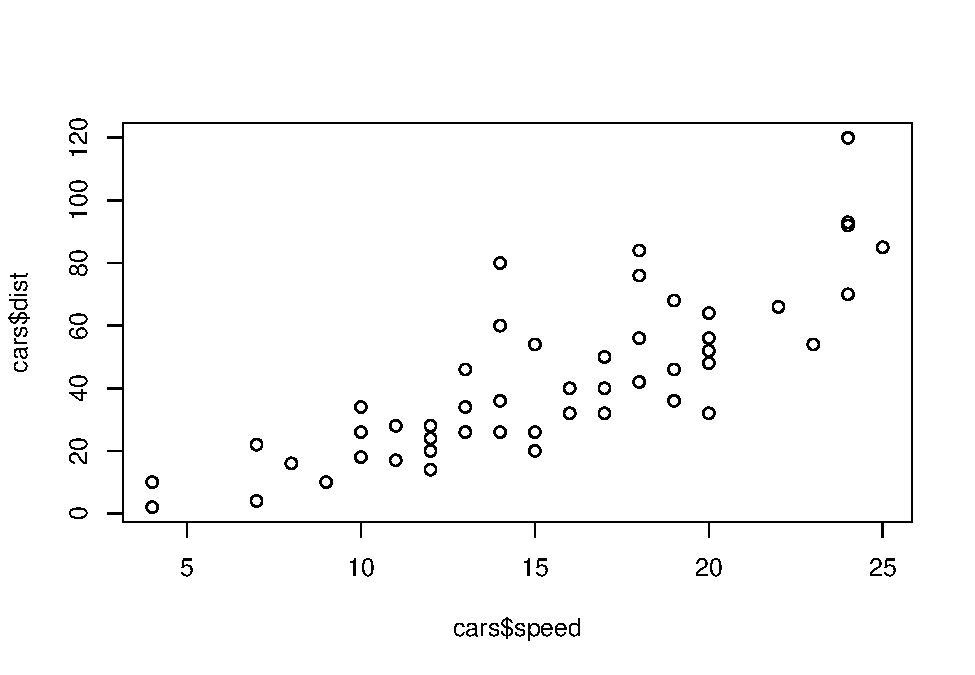
\includegraphics{paper_files/figure-latex/fig-1-1} 

}

\caption{Scatterplot of Speed and Distance}\label{fig:fig-1}
\end{figure}

But it turns out that it doesn't always work so well.

\hypertarget{ggplot2-graphs}{%
\subsection{ggplot2 graphs}\label{ggplot2-graphs}}

Same is true for ggplot2 as you can see in Figure \ref{fig:fig-2}.

\begin{Shaded}
\begin{Highlighting}[]
\NormalTok{mtcars}\OperatorTok{$}\NormalTok{cyl <-}\StringTok{ }\KeywordTok{as.factor}\NormalTok{(mtcars}\OperatorTok{$}\NormalTok{cyl) }\CommentTok{# Convert cyl to factor}
\KeywordTok{library}\NormalTok{(ggplot2)}
\KeywordTok{ggplot}\NormalTok{(mtcars, }\KeywordTok{aes}\NormalTok{(}\DataTypeTok{x=}\NormalTok{wt, }\DataTypeTok{y=}\NormalTok{mpg, }\DataTypeTok{shape=}\NormalTok{cyl)) }\OperatorTok{+}\StringTok{ }\KeywordTok{geom_point}\NormalTok{() }\OperatorTok{+}
\StringTok{  }\KeywordTok{labs}\NormalTok{(}\DataTypeTok{x=}\StringTok{"Weight (lb/1000)"}\NormalTok{, }\DataTypeTok{y =} \StringTok{"Miles/(US) gallon"}\NormalTok{, }
       \DataTypeTok{shape=}\StringTok{"Number of }\CharTok{\textbackslash{}n}\StringTok{ Cylinders"}\NormalTok{) }\OperatorTok{+}\StringTok{ }\KeywordTok{theme_classic}\NormalTok{()}
\end{Highlighting}
\end{Shaded}

\begin{figure}[H]

{\centering 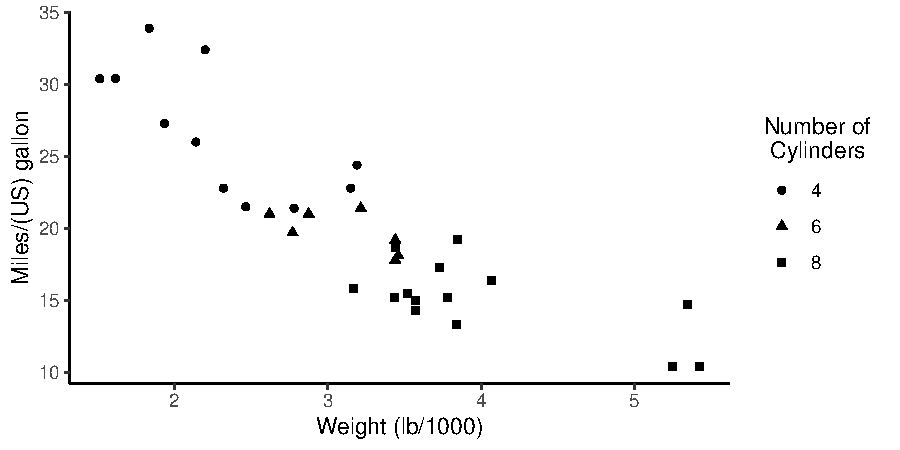
\includegraphics{paper_files/figure-latex/fig-2-1} 

}

\caption{Miles per gallon according to the weight}\label{fig:fig-2}
\end{figure}

\hypertarget{good-practices}{%
\section{Good practices}\label{good-practices}}

Every researcher has his own optimized setup. Currently I would recommend the following:

\begin{itemize}
\tightlist
\item
  Keep all files of your project (that matter for producing the PDF) in one folder without subfolders. You can zip and directly upload that folder to the \href{https://dataverse.harvard.edu/}{Harvard dataverse}.
\item
  Make sure that filenames have a logic to them.

  \begin{itemize}
  \tightlist
  \item
    Main file with text/code: ``paper.rmd'', ``report.rmd''
  \item
    Data files: "data\_xxxxxx.*"
  \item
    Image files: "fig\_xxxxxx.*"
  \item
    Tables files: "table\_xxxx.*"
  \item
    etc.
  \item
    Ideally, your filenames will correspond to the names in the paper. For instance, Figure 1 in the paper may have a corresponding file called \texttt{fig\_1\_xxxxx.pdf}.
  \end{itemize}
\item
  Use the document outline in R studio (Ctrl + Shift + O) when you work with R Markdown.
\item
  Name rchunks according to what they do or produce:

  \begin{itemize}
  \tightlist
  \item
    ``\texttt{fig-...}'' for chunks producing figures
  \item
    ``\texttt{table-...}'' for chunks producing tables
  \item
    ``\texttt{model-...}'' for chunks producing model estimates
  \item
    ``\texttt{import-...}'' for chunks importing data
  \item
    ``\texttt{recoding-...}'' for chunks in which data is recoded
  \end{itemize}
\item
  Use ``really'' informative variable names:

  \begin{itemize}
  \tightlist
  \item
    Q: What do you think does the variable \emph{trstep} measure? It actually measures trust in the European parliament.

    \begin{itemize}
    \tightlist
    \item
      How could we call this variable instead? Yes, \texttt{trust.european.parliament} which is longer but will probably be understood by another researcher.
    \end{itemize}
  \item
    If your setup is truly reproducible you will probably re-use the variable names that you generate as variable names in the tables you produce. Hence, there is an incentive to use good names.
  \end{itemize}
\item
  Use unique identifiers in the final document:

  \begin{itemize}
  \tightlist
  \item
    e.g., name the models you estimate ``M1'', ``M2'' etc.
  \item
    These unique names should also appear in the published paper.
  \item
    Think of someone who wants to produce Figure 1/Model 1 in your paper but doesn't find it in your code\ldots{}
  \end{itemize}
\end{itemize}

\hypertarget{additional-tricks-for-publishing}{%
\section{Additional tricks for publishing}\label{additional-tricks-for-publishing}}

\begin{itemize}
\tightlist
\item
  Make your script anonymous

  \begin{itemize}
  \tightlist
  \item
    Simply put a \texttt{\textless{}!-\/-\ ...\ -\/-\textgreater{}} around any identifying information, e.g., author names, title footnote etc.
  \end{itemize}
\item
  Counting words

  \begin{itemize}
  \tightlist
  \item
    Use adobe acrobat (commerical software) to convert your file to a word file. Then open in word and delete all the parts that shouldn't go into the word count. The word count is displayed in the lower right.
  \item
    Use an one of the online services to count your words (search for ``pdf word count'')
  \end{itemize}
\item
  Appendix: You can change the numbering format for the appendix in the rmd file

  \begin{itemize}
  \tightlist
  \item
    What is still not possible in this document is to automatically have separate reference sections for paper and appendix.
  \end{itemize}
\item
  Journals may require you to use their tex style: Sometimes you can simply use their template in your rmarkdown file. See \href{https://dataverse.harvard.edu/dataset.xhtml?persistentId=doi:10.7910/DVN/LDUMNY}{here} for a PLOS one example.
\end{itemize}

\hypertarget{citation-styles}{%
\section{Citation styles}\label{citation-styles}}

If your study needs to follow a particular citation style, you can set the corresponding style in the header of your \texttt{.rmd} document. To do so you have to download the corresponding \texttt{.csl} file.

In the present document we use the style of the American Sociological Association and set it in the preamble with \texttt{csl:\ american-sociological-association.csl}. However, you also need to download the respective \texttt{.csl} file from the following github page: \url{https://github.com/citation-style-language/styles} and copy it into your working directory for it to work.

The github directory contains a wide variety of citation style files depending on what discipline you work in.

\hypertarget{references}{%
\section{References}\label{references}}

\linespread{1}

\hypertarget{refs}{}
\leavevmode\hypertarget{ref-markdown2017}{}%
Allaire, JJ, Jeffrey Horner, Vicent Marti, and Natacha Porte. 2017. \emph{Markdown: 'Markdown' Rendering for R}.

\leavevmode\hypertarget{ref-hlavac2013stargazer}{}%
Hlavac, Marek. 2013. ``Stargazer: LaTeX Code and Ascii Text for Well-Formatted Regression and Summary Statistics Tables.'' \emph{URL: Http://CRAN. R-Project. Org/Package= Stargazer}.

\leavevmode\hypertarget{ref-Kirsop2005-ro}{}%
Kirsop, Barbara and Leslie Chan. 2005. ``Transforming Access to Research Literature for Developing Countries.'' \emph{Serials Review} 31(4):246--55.

\leavevmode\hypertarget{ref-R2017}{}%
R Core Team. 2017. \emph{R: A Language and Environment for Statistical Computing}. Vienna, Austria: R Foundation for Statistical Computing.

\leavevmode\hypertarget{ref-Rstudio2015}{}%
RStudio Team. 2015. \emph{RStudio: Integrated Development Environment for R}. Boston, MA: RStudio, Inc.

\leavevmode\hypertarget{ref-plotly}{}%
Sievert, Carson, Chris Parmer, Toby Hocking, Scott Chamberlain, Karthik Ram, Marianne Corvellec, and Pedro Despouy. 2017. \emph{Plotly: Create Interactive Web Graphics via 'Plotly.js'}.

\leavevmode\hypertarget{ref-knitr3}{}%
Xie, Yihui. 2014. ``Knitr: A Comprehensive Tool for Reproducible Research in R.'' in \emph{Implementing reproducible computational research}, edited by V. Stodden, F. Leisch, and R. D. Peng. Chapman; Hall/CRC.

\leavevmode\hypertarget{ref-knitr2}{}%
Xie, Yihui. 2015. \emph{Dynamic Documents with R and Knitr}. 2nd ed. Boca Raton, Florida: Chapman; Hall/CRC.

\leavevmode\hypertarget{ref-bookdown2}{}%
Xie, Yihui. 2016. \emph{Bookdown: Authoring Books and Technical Documents with R Markdown}. Boca Raton, Florida: Chapman; Hall/CRC.

\leavevmode\hypertarget{ref-bookdown1}{}%
Xie, Yihui. 2017. \emph{Bookdown: Authoring Books and Technical Documents with R Markdown}.

\leavevmode\hypertarget{ref-knitr1}{}%
Xie, Yihui. 2018a. \emph{Knitr: A General-Purpose Package for Dynamic Report Generation in R}.

\leavevmode\hypertarget{ref-tinytex}{}%
Xie, Yihui. 2018b. \emph{Tinytex: Helper Functions to Install and Maintain 'Tex Live', and Compile 'Latex' Documents}.

\leavevmode\hypertarget{ref-kableextra}{}%
Zhu, Hao. 2017. \emph{KableExtra: Construct Complex Table with 'Kable' and Pipe Syntax}.

\clearpage

\appendix
\addtocontents{toc}{\protect\setcounter{tocdepth}{2}}

\renewcommand{\thesection}{A}

\setcounter{page}{1}

\setcounter{table}{0}
\renewcommand{\thetable}{A\arabic{table}}
\renewcommand{\figurename}{Table}

\setcounter{figure}{0}
\renewcommand\thefigure{A\arabic{figure}}
\renewcommand{\figurename}{Figure}

\clearpage
\pagenumbering{gobble}

\vspace*{7cm}

\begin{center}
\begin{huge}
Online Appendix
\end{huge}
\end{center}
\vspace{3cm}

\clearpage
\pagenumbering{arabic}

\hypertarget{online-appendix}{%
\section{Online appendix}\label{online-appendix}}

\hypertarget{sec:rsessioninfo}{%
\subsection{Attach R session info in appendix}\label{sec:rsessioninfo}}

Since R and R packages are constantly evolving you might want to add the R session info that contains information on the R version as well as the packages that are loaded.

\begin{verbatim}
## R version 4.0.3 (2020-10-10)
## Platform: x86_64-apple-darwin17.0 (64-bit)
## Running under: macOS Big Sur 10.16
## 
## Matrix products: default
## BLAS:   /Library/Frameworks/R.framework/Versions/4.0/Resources/lib/libRblas.dylib
## LAPACK: /Library/Frameworks/R.framework/Versions/4.0/Resources/lib/libRlapack.dylib
## 
## attached base packages:
## [1] stats     graphics  grDevices utils     datasets  methods   base     
## 
## other attached packages:
## [1] ggplot2_3.3.3    kableExtra_1.3.1 knitr_1.30       stargazer_5.2.2 
## 
## loaded via a namespace (and not attached):
##  [1] compiler_4.0.3    pillar_1.5.1      tools_4.0.3       digest_0.6.27    
##  [5] evaluate_0.14     lifecycle_1.0.0   tibble_3.1.0      gtable_0.3.0     
##  [9] viridisLite_0.3.0 pkgconfig_2.0.3   rlang_0.4.10      DBI_1.1.0        
## [13] rstudioapi_0.13   yaml_2.2.1        xfun_0.19         withr_2.4.1      
## [17] httr_1.4.2        stringr_1.4.0     dplyr_1.0.5       xml2_1.3.2       
## [21] generics_0.1.0    vctrs_0.3.6       tidyselect_1.1.0  webshot_0.5.2    
## [25] grid_4.0.3        glue_1.4.2        R6_2.5.0          fansi_0.4.2      
## [29] rmarkdown_2.6     bookdown_0.21     farver_2.1.0      purrr_0.3.4      
## [33] magrittr_2.0.1    scales_1.1.1      htmltools_0.5.1.1 ellipsis_0.3.1   
## [37] assertthat_0.2.1  rvest_0.3.6       colorspace_2.0-0  labeling_0.4.2   
## [41] utf8_1.2.1        stringi_1.5.3     munsell_0.5.0     crayon_1.4.1
\end{verbatim}

\hypertarget{all-the-code-in-the-paper}{%
\subsection{All the code in the paper}\label{all-the-code-in-the-paper}}

To simply attach all the code you used in the PDF file in the appendix see the R chunk in the underlying \texttt{.rmd} file:

\begin{Shaded}
\begin{Highlighting}[]
\NormalTok{knitr}\OperatorTok{::}\NormalTok{opts_chunk}\OperatorTok{$}\KeywordTok{set}\NormalTok{(}\DataTypeTok{cache =} \OtherTok{FALSE}\NormalTok{)}
\CommentTok{# Use chache = TRUE if you want to speed up compilation}

\CommentTok{# A function to allow for showing some of the inline code}
\NormalTok{rinline <-}\StringTok{ }\ControlFlowTok{function}\NormalTok{(code)\{}
\NormalTok{  html <-}\StringTok{ '<code  class="r">``` `r CODE` ```</code>'}
  \KeywordTok{sub}\NormalTok{(}\StringTok{"CODE"}\NormalTok{, code, html)}
\NormalTok{\}}
\KeywordTok{install.packages}\NormalTok{(}\KeywordTok{c}\NormalTok{(}\StringTok{'tinytex'}\NormalTok{, }\StringTok{'rmarkdown'}\NormalTok{))}
\NormalTok{tinytex}\OperatorTok{::}\KeywordTok{install_tinytex}\NormalTok{()}
\KeywordTok{install.packages}\NormalTok{(}\KeywordTok{c}\NormalTok{(}\StringTok{"rmarkdown"}\NormalTok{, }\StringTok{"knitr"}\NormalTok{, }\StringTok{"kableExtra"}\NormalTok{,}
                   \StringTok{"stargazer"}\NormalTok{, }\StringTok{"plotly"}\NormalTok{, }\StringTok{"knitr"}\NormalTok{,}
                   \StringTok{"bookdown"}\NormalTok{))}
\KeywordTok{cat}\NormalTok{(}\KeywordTok{paste}\NormalTok{(}\StringTok{"#"}\NormalTok{, }\KeywordTok{capture.output}\NormalTok{(}\KeywordTok{sessionInfo}\NormalTok{()), }\StringTok{"}\CharTok{\textbackslash{}n}\StringTok{"}\NormalTok{, }\DataTypeTok{collapse =}\StringTok{""}\NormalTok{)) }
  \CommentTok{# or use message() instead of cat()}
\NormalTok{data <-}\StringTok{ }\KeywordTok{read.csv}\NormalTok{(}\StringTok{"data.csv"}\NormalTok{)}
\KeywordTok{head}\NormalTok{(data)}
\KeywordTok{dput}\NormalTok{(data)}
\NormalTok{data <-}\StringTok{ }\KeywordTok{structure}\NormalTok{(}\KeywordTok{list}\NormalTok{(}\DataTypeTok{X =} \DecValTok{1}\OperatorTok{:}\DecValTok{50}\NormalTok{, }\DataTypeTok{speed =} \KeywordTok{c}\NormalTok{(4L, 4L, 7L, 7L, 8L, 9L, 10L, }
\NormalTok{10L, 10L, 11L, 11L, 12L, 12L, 12L, 12L, 13L, 13L, 13L, 13L, 14L, }
\NormalTok{14L, 14L, 14L, 15L, 15L, 15L, 16L, 16L, 17L, 17L, 17L, 18L, 18L, }
\NormalTok{18L, 18L, 19L, 19L, 19L, 20L, 20L, 20L, 20L, 20L, 22L, 23L, 24L, }
\NormalTok{24L, 24L, 24L, 25L), }\DataTypeTok{dist =} \KeywordTok{c}\NormalTok{(2L, 10L, 4L, 22L, 16L, 10L, 18L, }
\NormalTok{26L, 34L, 17L, 28L, 14L, 20L, 24L, 28L, 26L, 34L, 34L, 46L, 26L, }
\NormalTok{36L, 60L, 80L, 20L, 26L, 54L, 32L, 40L, 32L, 40L, 50L, 42L, 56L, }
\NormalTok{76L, 84L, 36L, 46L, 68L, 32L, 48L, 52L, 56L, 64L, 66L, 54L, 70L, }
\NormalTok{92L, 93L, 120L, 85L)), }
\DataTypeTok{class =} \StringTok{"data.frame"}\NormalTok{, }\DataTypeTok{row.names =} \KeywordTok{c}\NormalTok{(}\OtherTok{NA}\NormalTok{, }
\OperatorTok{-}\NormalTok{50L))}
\KeywordTok{library}\NormalTok{(stargazer)}
\KeywordTok{stargazer}\NormalTok{(cars, }
          \DataTypeTok{title =} \StringTok{"Summary table with stargazer"}\NormalTok{,}
          \DataTypeTok{label=}\StringTok{"tab1"}\NormalTok{, }
          \DataTypeTok{table.placement =} \StringTok{"H"}\NormalTok{, }
          \DataTypeTok{header=}\OtherTok{FALSE}\NormalTok{)}
\KeywordTok{library}\NormalTok{(stargazer)}
\NormalTok{model1 <-}\StringTok{ }\KeywordTok{lm}\NormalTok{(speed }\OperatorTok{~}\StringTok{ }\NormalTok{dist, }\DataTypeTok{data =}\NormalTok{ cars)}
\NormalTok{model2 <-}\StringTok{ }\KeywordTok{lm}\NormalTok{(speed }\OperatorTok{~}\StringTok{ }\NormalTok{dist, }\DataTypeTok{data =}\NormalTok{ cars)}
\NormalTok{model3 <-}\StringTok{ }\KeywordTok{lm}\NormalTok{(dist }\OperatorTok{~}\StringTok{ }\NormalTok{speed, }\DataTypeTok{data =}\NormalTok{ cars)}
\KeywordTok{stargazer}\NormalTok{(model1, model2, model3,}
          \DataTypeTok{title =} \StringTok{"Regression table with stargazer"}\NormalTok{,}
          \DataTypeTok{label=}\StringTok{"tab2"}\NormalTok{, }
          \DataTypeTok{table.placement =} \StringTok{"H"}\NormalTok{, }
          \DataTypeTok{column.labels =} \KeywordTok{c}\NormalTok{(}\StringTok{"M1"}\NormalTok{, }\StringTok{"M2"}\NormalTok{, }\StringTok{"M3"}\NormalTok{),}
          \DataTypeTok{model.numbers =} \OtherTok{FALSE}\NormalTok{,}
          \DataTypeTok{header=}\OtherTok{FALSE}\NormalTok{)}
\KeywordTok{library}\NormalTok{(knitr)}
\KeywordTok{library}\NormalTok{(kableExtra)}
\KeywordTok{kable}\NormalTok{(cars[}\DecValTok{1}\OperatorTok{:}\DecValTok{10}\NormalTok{,], }\DataTypeTok{row.names =} \OtherTok{TRUE}\NormalTok{, }
      \DataTypeTok{caption =} \StringTok{'Table with kable() and kablestyling()'}\NormalTok{, }
      \DataTypeTok{format =} \StringTok{"latex"}\NormalTok{, }\DataTypeTok{booktabs =}\NormalTok{ T) }\OperatorTok
\StringTok{        }\KeywordTok{kable_styling}\NormalTok{(}\DataTypeTok{full_width =}\NormalTok{ T, }
                      \DataTypeTok{latex_options =} \KeywordTok{c}\NormalTok{(}\StringTok{"striped"}\NormalTok{, }
                                        \StringTok{"scale_down"}\NormalTok{,}
                                        \StringTok{"HOLD_position"}\NormalTok{),}
                      \DataTypeTok{font_size =} \DecValTok{10}\NormalTok{)}
\KeywordTok{plot}\NormalTok{(cars}\OperatorTok{$}\NormalTok{speed, cars}\OperatorTok{$}\NormalTok{dist)}
\NormalTok{mtcars}\OperatorTok{$}\NormalTok{cyl <-}\StringTok{ }\KeywordTok{as.factor}\NormalTok{(mtcars}\OperatorTok{$}\NormalTok{cyl) }\CommentTok{# Convert cyl to factor}
\KeywordTok{library}\NormalTok{(ggplot2)}
\KeywordTok{ggplot}\NormalTok{(mtcars, }\KeywordTok{aes}\NormalTok{(}\DataTypeTok{x=}\NormalTok{wt, }\DataTypeTok{y=}\NormalTok{mpg, }\DataTypeTok{shape=}\NormalTok{cyl)) }\OperatorTok{+}\StringTok{ }\KeywordTok{geom_point}\NormalTok{() }\OperatorTok{+}
\StringTok{  }\KeywordTok{labs}\NormalTok{(}\DataTypeTok{x=}\StringTok{"Weight (lb/1000)"}\NormalTok{, }\DataTypeTok{y =} \StringTok{"Miles/(US) gallon"}\NormalTok{, }
       \DataTypeTok{shape=}\StringTok{"Number of }\CharTok{\textbackslash{}n}\StringTok{ Cylinders"}\NormalTok{) }\OperatorTok{+}\StringTok{ }\KeywordTok{theme_classic}\NormalTok{()}
\KeywordTok{print}\NormalTok{(}\KeywordTok{sessionInfo}\NormalTok{(), }\DataTypeTok{local =} \OtherTok{FALSE}\NormalTok{)}
\end{Highlighting}
\end{Shaded}

\end{document}
